\documentclass{beamer}
\usepackage{listings}
%
% Choose how your presentation looks.
%
% For more themes, color themes and font themes, see:
% http://deic.uab.es/~iblanes/beamer_gallery/index_by_theme.html
%
\mode<presentation>
{
  \usetheme{default}      % or try Darmstadt, Madrid, Warsaw, ...
  \usecolortheme{default} % or try albatross, beaver, crane, ...
  \usefonttheme{default}  % or try serif, structurebold, ...
  \setbeamertemplate{navigation symbols}{}
  \setbeamertemplate{caption}[numbered]
} 

\usepackage[english]{babel}
\usepackage[utf8x]{inputenc}

\title[]{Forensic Analysis of Web Data}
\author{Erhard Dinhobl}
\institute{Vienna University of Technology - Information and Software Engineering Group}
\date{5.10.2016}

\begin{document}

\begin{frame}
  \titlepage
\end{frame}

% Uncomment these lines for an automatically generated outline.
%\begin{frame}{Outline}
%  \tableofcontents
%\end{frame}

\begin{frame}{Introduction}

\begin{itemize}
  \item using collected data in surveys
  \item influence to known investigative models
  \item appropriate investigation model
  \item digital preservation
  \item legal issues
  \item deep web crawling
  \item format of data
  \item designing a deep web crawler
\end{itemize}

\end{frame}

\begin{frame}{Table of contents}

\begin{itemize}
  \item base investigation model
  \item new investigation model
  \item "reduct", "preserve" and "analyze" steps in detail
  \item underlying methodology (deep web crawler)
  \item usage
\end{itemize}
\end{frame}


\begin{frame}{The Investigation S(RP)AP}
\begin{itemize}
  \item secure
  \item \textbf{reduct}
  \item \textbf{preserve}
  \item analyze
  \item present
\end{itemize}

Best for online crime investigation!

\end{frame}

\begin{frame}{The Process}

\begin{figure}
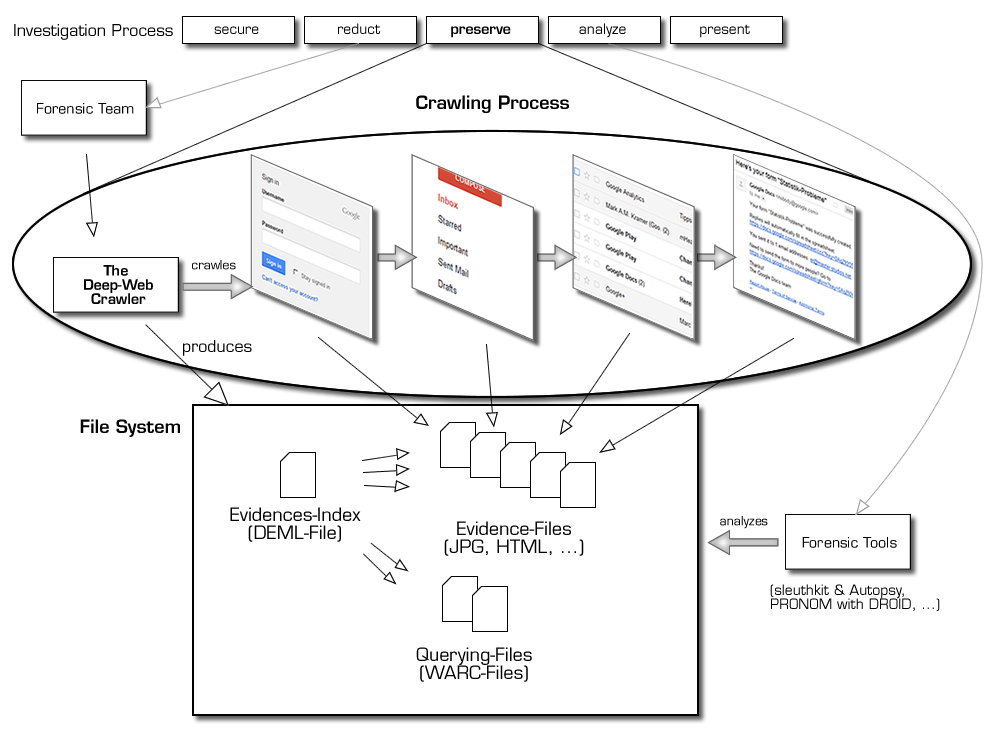
\includegraphics[scale=0.3]{figure-1.png}
\end{figure}

\end{frame}

\begin{frame}{The Process (2)}

\begin{itemize}
  \item Where was the evidence stored?
  \item Who had obtained the evidence?
  \item What has been done to the evidence?
\end{itemize}

\end{frame}

\begin{frame}{"reduct"}

\begin{itemize}
  \item reduce amount of data to crawl (also time)
  \item crawling websites: XPath
  \item simulate user navigation and interaction
  \item defined by investigation team
  \item be aware: unimportant data maybe later important
\end{itemize}

\end{frame}

\begin{frame}{"preserve"}

\begin{itemize}
  \item preservation of evidences up to 60 years (StPO \S60)
  \item important due to file formats (determined with DROID)
  \item for web crawling WARC file format (open format)
  \item for immediate investigation: normal files
  \item the index: DEML file
  \begin{itemize}
    \item by National Centre for Forensic Science
    \item Digital Evidence Markup Language
    \item compatible with Global Justice XML Data Model (GJXDM)
    \item File (inheritance: DigitalArtefact, Allocated) important for online investigations
  \end{itemize}
\end{itemize}

\end{frame}

\begin{frame}{"analyze"}

\begin{itemize}
  \item file analysis: sleuthkit, Autopsy, PRONOM (with DROID)
  \item own tools and usage of graph-expression (Google)
  \item timeline and correlation reconstruction:
  \begin{itemize}
  	\item model from the National Centre for Forensic Science
	\item Application, Content, Principal, System
  \end{itemize}
\end{itemize}

\begin{figure}
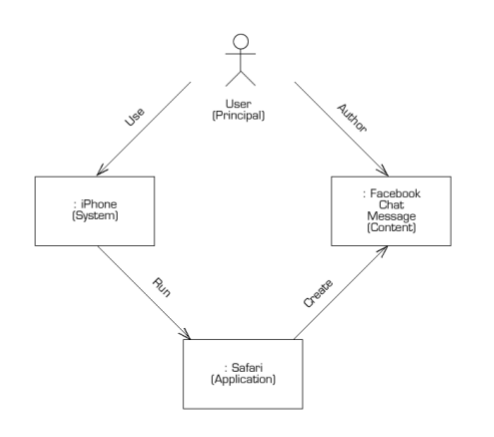
\includegraphics[scale=0.4]{model2.png}
\end{figure}

\end{frame}

\begin{frame}{The Deep Web Crawler}

Challenges:

\begin{itemize}
  \item the use of AJAX technology in web pages
  \item the simulation of user interaction with HTML elements (e.g. forms)
  \item the use of Captchas in web pages
\end{itemize}

\end{frame}

\begin{frame}{The Architecture}

\begin{figure}
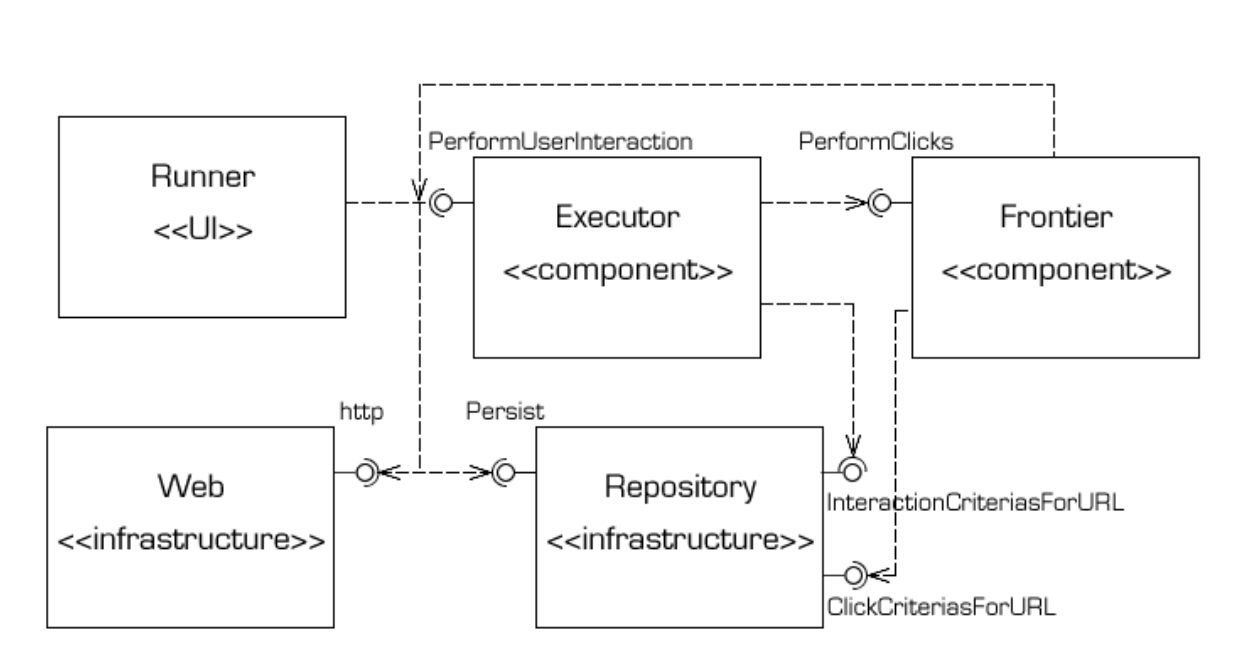
\includegraphics[scale=0.2]{crawler-deepweb-componentdiagram.png}
\end{figure}

\end{frame}


\defverbatim[colored]\lst{%
\begin{lstlisting}[tabsize=8,basicstyle=\ttfamily]

<?xml version="1.0"?>
<cratalis start-url="http://kurier.at" 
    name="Kurier Crawling" 
    start-action-sequence="1">
  <action-sequence id="1">
    <action type="StartAction" id="1" 
        comment="start every link" save="true" 
	action-sequence-id="3">
	  .//a[@href and 
	  not(starts-with(@href, "#"))]
    </action>
  </action-sequence>
  <action-sequence id="3">
    <action type="SaveAction" id="3" 
        comment="just save" save="true"/>
  </action-sequence>
</cratalis>

\end{lstlisting}
}

\begin{frame}{Simple Example}
\lst
\end{frame}


\defverbatim[colored]\lst{%
\begin{lstlisting}[tabsize=8,basicstyle=\tiny]

<?xml version="1.0"?>
<cratalis start-url="http://www.studivz.de" name="StudiVZ" start-action-sequence="1" 
      deml-file="studivz/studivz.xml">
  <action-sequence id="1">
    <action type="JavaScript" id="1" comment="filling out the login form" 
          save="true" save-file="studivz/login-screen.html">
        var usernameInputs = document.evaluate(".//*[@id='Login_email']", ...);
        var usernameTextBox = usernameInputs.iterateNext();
        usernameTextBox.value = "forensicanalysis@ymail.com";
        var passwordInputs = document.evaluate(".//*[@id='Login_password']", ...);
        var passwordTextBox = passwordInputs.iterateNext();
        passwordTextBox.value = "gustav";
    </action>
    <action type="StartAction" id="2" save-file="studivz/home.html"....></action>
  </action-sequence>
  <action-sequence id="2">
    <action type="StartAction" id="3" save-file="studivz/inbox.html"></action>
  </action-sequence>
  <action-sequence id="3">
    <action type="JavaScript" id="4" comment="start other action to overview" ...>
        var msgLinkList = document.evaluate(
	      ".//div[contains(@class,'from-subject')]/.../a", ...);
        var msgLink;
        var count = 0;
        while(msgLink = msgLinkList.iterateNext()) {
            count++;
            msgLink.onclick.apply(msgLink);
            savePage('studivz/msg' + count + '.html');
        }
    </action>
  </action-sequence>
</cratalis>

\end{lstlisting}
}

\begin{frame}{More complex example}
\lst
\end{frame}

\begin{frame}{Usage}

\begin{itemize}
  \item investigative
  \begin{itemize}
    \item collecting bitcoin addresses (clear and dark net)
    \item saving evidence files from the web (also via Tor)
  \end{itemize}

  \item non-investigative
  \begin{itemize}
    \item collecting event data
    \item ... market watch
    \item ... person data (incl. relations)
    \item ... news
    \item ... locations
    \item ... bitcoin addresses and names
    \item many others still done
  \end{itemize}
\end{itemize}

\end{frame}

\end{document}
